\documentclass{article}

\usepackage{amsmath,amssymb,amsthm}
\usepackage{graphics,tikz}
\setlength{\oddsidemargin}{0.25 in}
\setlength{\evensidemargin}{-0.25 in}
\setlength{\topmargin}{-0.6 in}
\setlength{\textwidth}{6.5 in}
\setlength{\textheight}{8.5 in}
\setlength{\headsep}{0.75 in}
\setlength{\parindent}{0 in}
\setlength{\parskip}{0.1 in}

\newtheorem{theorem}{Theorem}
\newtheorem{corollary}{Corollary}
\newtheorem{proposition}{Proposition}
\newtheorem*{remark}{Remark}
\theoremstyle{definition}
\newtheorem{example}{Example}
\newtheorem{definition}{Definition}

\newcommand{\lecture}[4]{
   \pagestyle{myheadings}
   \thispagestyle{plain}
   \newpage
%   \setcounter{lecnum}{#1}
   \setcounter{page}{1}
   \noindent
   \begin{center}
   \framebox{
      \vbox{\vspace{2mm}
    \hbox to 6.58in { {\bf CSC~565: Graph Theory
                        \hfill North Carolina State University} }
    \hbox to 6.58in { {\bf Fall 2019
                        \hfill Computer Science} }
       \vspace{4mm}
       \hbox to 6.28in { {\Large \hfill Lecture #1: #2  \hfill} }
       \vspace{2mm}
       \hbox to 6.28in { {\it Lecturer: {\it Don Sheehy {\tt <drsheehy@ncsu.edu>}} \hfill Scribe: #4} }
      \vspace{2mm}}
   }
   \end{center}
   \markboth{Lecture #1: #2}{Lecture #1: #2}
   \vspace*{4mm}
}

\def\geom{\text{geom}}
\def\R{\mathbb{R}}

\begin{document}


%FILL IN THE RIGHT INFO.
%\lecture{**LECTURE-NUMBER**}{**DATE**}{**LECTURER**}{**SCRIBE**}
\lecture{4}{Sep 4, 2019}{Don Sheehy}{Cash Bortner and Ran Tan}

  % \title{Lecture 4}
  % \author{Scribed by: Cash Bortner and Ran Tan}
  % \maketitle

  \begin{theorem}
  If $G$ is isomorphic to $H$, i.e $G \cong H$, then the set of edges of $G$ has the same cardinality as the set of edges of $H$, i.e. $|E_G|=|E_H|$.
  \end{theorem}
  \begin{proof}[Proof idea]
  Recall that two graphs are \textit{isomorphic} if there exists a bijective morphism between them, i.e. there exists a bijective function from the vertex set of one graph to the vertex set of the other such that edges in the first graph map to edges in the second graph.  We can formalize the idea of isomorphism between the graphs $G$ and $H$, as a bijective function $f \colon G \to H$ where really the function $f$ is defined on the vertex sets: $f\colon V_G \to V_H$ where if $(u,v) \in E_G$, then $\big(f(u),f(v)\big) \in E_H$.  Via a categorical function which maps a graph to its sets of edges, we can also consider the induced bigjective function $f_1 \colon E_G \to E_H$ defined as $f_1(a,b) = \big( f(a) , f(b) \big)$.
  \[\begin{array}{rccccc}
      &\text{Graphs}&\hspace*{5mm} &G & \overset{f}{\underset{f^{-1}}{\scalebox{3}[1.5]{\ensuremath{\rightleftarrows}}}}& H \\
     \text{functor}&\scalebox{1.5}[3]{\ensuremath{\downarrow}} &&\scalebox{1.5}[3]{\ensuremath{\downarrow}} && \scalebox{1.5}[3]{\ensuremath{\downarrow}}\\
      &\text{Sets} &&E_G & \overset{f_1}{\underset{f_1^{-1}}{\scalebox{3}[1.5]{\ensuremath{\rightleftarrows}}}}& E_H \\
  \end{array}\]
  This induced map $f_1$ is also bijective, hence the domain and codomain must have the same cardinality, i.e. $|E_G| = |E_H|$ as desired.
  \end{proof}


We can now consider morphisms from specific graphs, for example $C_n$ and $P_m$, i.e. the cycle with $n$ edges [and vertices] and the path with $m$ edges [and $m+1$ vertices] respectively.  

If we first consider any morphism from $P_m$ to a general graph $G$, the image of said morphism will always yield a \textit{walk} in $G$, i.e. a sequence of vertices $(v_0, v_1 , \ldots, v_m) \subseteq V_G$ such that $(v_{i-1},v_{i}) \in E_G$ for each $i=1,\ldots m$.  On the other hand, if the morphism from $P_m$ to $G$ is injective, the image yields a \textit{path} in $G$, i.e. a walk such that none of the vertices are repeated.

If we now consider any morphism from $C_n$ to a general graph $G$, the image of said morphism will always yield a \textit{tour}, i.e. a walk such that you end at the vertex that you started at.  If the morphism from $C_n$ to $G$ is injective, the image yields a \textit{cycle}, i.e. a tour with no repeated vertices other than the first and last.

Consider the following example:

\begin{example}
Consider the graph defined by $V=\{a,b,c,d,e\}$ and $E=\big\lbrace \{a,b\},\{b,c\},\{a,c\},\{c,d\},\{d,e\},\{a,e\} \big\rbrace$.  Suppose we wanted to find the cycles of length four in this graph $G=(V,E)$.  From the above remark, we can consider the images of the injective maps from $C_4$ to $G$ to find the cycles, in $G$.  In this case, up to renaming the vertices, there is only one injective map from $C_4$ to $G$, namely the map (up to permutations):
\begin{align*}
    1 &\mapsto c \\
    2 &\mapsto d \\
    3 &\mapsto e \\
    4 &\mapsto a 
\end{align*}
Thus, there is only one cycle up to permuting the the vertices in $G$.

\begin{center}
\begin{tikzpicture}[every node/.style={draw,circle,minimum size=7mm}]
%C_4

\node (1) at (-11,1) {1};
\node (2) at (-8,1) {2};
\node (3) at (-8,4) {3};
\node (4) at (-11,4) {4};

\draw[thick] (1) -- (2) -- (3) -- (4) -- (1);

\node[draw=none] at (-5.75,2.5) {$\scalebox{7}[4]{\ensuremath{\hookrightarrow}}$};

%Graph G
\node (a) at (0,5) {$a$};
\node (b) at (-3,3) {$b$};
\node (c) at (-2,0) {$c$};
\node (d) at (2,0) {$d$};
\node (e) at (3,3) {$e$};

\draw[thick] (a) -- (b) 
      (b) -- (c) 
      (c) -- (d)
      (d) -- (e)
      (e) -- (a) 
      (a) -- (c);
      
\node[draw=none] at (-9.5,0) {$C_4$};
\node[draw=none] at (0,-1) {$G$};

\draw[->, dashed,red] (-10.7,0.7) .. controls (-8,-2) and (-5,-2) .. (-2.3,-.4);
\draw[->, dashed,red] (-7.7,0.7) .. controls (-5,-2) and (-3,-2) .. (1.7,-.3);
\draw[->, dashed,red] (-10.7,4.3) .. controls (-7,6) and (-3,6) .. (-.3,5.3);
\draw[->, dashed,red] (-7.7,4.3) .. controls (-3,7) and (1,6.5) .. (2.9,3.4);

\end{tikzpicture}
\end{center}
\end{example}

\section{Geometric Realization of Graph}
\begin{example}
Consider a path in the plane 
\begin{center}
    \begin{tikzpicture}
    \node (1) at (-0.5,0) {0};
    \node (2) at (4.5,1) {1};
    
    \draw[thick] (0,0) .. controls (1,2) and (2,0) .. (4,1);
    \end{tikzpicture}\\  
\end{center}

and think of it as a set of points in the plane. If the path was traced out in time, the underlying function can be described as:\\
\begin{equation*}
    f: [0, 1] \rightarrow {\mathbb{R}}^2
\end{equation*}

\begin{center}
    \begin{tikzpicture}
    \node (1) at (0,-0.5) {f(0)};
    \node (2) at (4,0.5) {f(1)};
    \node (3) at (-4,-0.5) {0};
    \node (4) at (-2,-0.5) {1};
    \node (5) at (-3,-0.5) {$\frac{1}{2}$};
    \node (6) at (1,0.5) {$f(\frac{1}{2})$};
    
    \draw[thick] (-4,0) -- (-2, 0);
    \draw[thick] (0,0) .. controls (1,2) and (2,0) .. (4,1);
    \draw[->, dashed] (-4,0) .. controls (-3,1) .. (0,0);
    \draw[->, dashed] (-2,0) .. controls (0,2) .. (4,1);
    \draw[->, dashed] (-3,0) .. controls (-1,2) .. (1,1);
    \end{tikzpicture}\\  
\end{center}
This function $f$ allows us to label start and end, compute velocity, and trace the path. Here, we argue that the mapping is more important than its image. This naturally leads to the geometric realization of graphs.
\end{example}

Let $G=(V,E)$ be a graph with $|V|=n$.  We're going to consider the map $\phi \colon V \to \R^n$ defined by mapping each vertex to the standard basis vectors, i.e.
\[
\phi(v_i)  = b_i := \begin{bmatrix} 0 \\ \vdots \\ 0 \\ 1 \\ 0 \\ \vdots \\ 0 
\end{bmatrix}
\leftarrow i^{\text{th}} \text{ row.}
\]
This map $\phi$ sends edges to the convex combinations of the corresponding standard basis vectors, i.e. 
\[
(v_i,v_j) \in E_G \longmapsto \overline{b_ib_j}:= f(t)= (1-t)b_i + tb_j \hspace{1cm} \text{for all }t\in[0,1].
\]
This convex combination can be thought of geometrically as the line segment between [the ends of the basis vectors] $b_i$ and $b_j$.  

\begin{definition}
We now define the \textit{geometric realization} of a graph $G$ as
\[
\geom(G) := \left( \bigcup_{i=1}^n b_i \right) \ \bigcup \ \left( \bigcup_{(v_i,v_j) \in E_G} \overline{b_i b_j} \right) 
\]
\end{definition}








\begin{example}
Consider a geometric realization of graph $G = (\{v_1, v_2, v_3\}, \{(v_2, v_3)\})$ in $\mathbb{R}^3$\\
\begin{center}
    \begin{tikzpicture}[x=1cm, y=1cm, z=-0.5cm]
        % Axes
        \draw [->] (0,0,0) -- (4,0,0) node [at end, right] {$x$};
        \draw [->] (0,0,0) -- (0,4,0) node [at end, left] {$y$};
        \draw [->] (0,0,0) -- (0,0,4) node [at end, left] {$z$};
    
        % Vectors
        \draw [thick] (0,2,0) -- (0,0,2);
    
        % Labels
        \node [fill,circle, scale=0.3, label={above:$b_1$}] (1) at (2,0,0) {};
        \node [fill,circle, scale=0.3, label={left:$b_2$}] (2) at (0,2,0) {};
        \node [fill,circle, scale=0.3, label={left:$b_3$}] (3) at (0,0,2) {};
        \node (4) at (-1,1,1) {$\overline{b_2b_3}$};
    \end{tikzpicture}
\end{center}
\end{example}

In our definition, the image of map $\phi$ is a subset of $\mathbb{R}^n$. Let $\geom(G)$ be a geometric realization of $G$. All such subsets form a category. We can simply define any continuous map between these subsets to be a morphism. By definition, continuous means that preimage of open sets are open. In particular, note that
\begin{enumerate}
    \item Identity functions are continuous.
    \item Compositions of continuous functions are continuous. 
\end{enumerate}
The category $Top$ is defined as the sets of topological spaces and continuous maps between them.

\begin{definition}
A \textit{plane drawing} of graph $G$ is a continuous map 
\begin{equation*}
    \geom(G) \to \mathbb{R}^2
\end{equation*}
\end{definition}

\begin{definition}
An \textit{embedding} of graph $G$ is an injective map 
\begin{equation*}
    \geom(G) \hookrightarrow \mathbb{R}^2
\end{equation*}
\end{definition}

\begin{example}
Consider graphs $A$ and $B$ under different perspectives

\begin{center}
    \begin{tikzpicture}[]
    
    \node[draw,circle,minimum size=7mm] (1) at (-4,0) {1};
    \node[draw,circle,minimum size=7mm] (2) at (-2,2) {2};
    \node[draw,circle,minimum size=7mm] (3) at (0,0) {3};
    
    \draw[thick] (1) -- (2) -- (3);
    \node at (-2,-1) {$A$};
    
    \node[draw,circle,minimum size=7mm] (4) at (2,1) {$u$};
    \node[draw,circle,minimum size=7mm] (5) at (6,1) {$v$};
    
    \draw[thick] (4) -- (5);
    \node at (4,-1) {$B$};
    
    \node[draw=none] at (-2,-3) {$\scalebox{2}[6]{\ensuremath{\downarrow}}$};
    \node[draw=none] at (4,-3) {$\scalebox{2}[6]{\ensuremath{\downarrow}}$};

    \end{tikzpicture}
    
    
    \begin{tikzpicture}[]
    
    \node (1) at (-4,0) {1};
    \node (2) at (-2,2.3) {2};
    \node (3) at (0,0) {3};
    
    \draw[thick] (1) -- (-2,2) -- (3);
    \node at (-2,-1) {$\geom(A)$};
    
    \node (4) at (2,1) {$u$};
    \node (5) at (6,1) {$v$};
    
    \draw[thick] (4) -- (5);
    \node at (4,-1) {$\geom(B)$};
    
    \draw[red,<->,dashed] (-3.7,0.1) .. controls (-2.2,-2) and (0,-2) .. (2.2,.8);
    \draw[red,<->,dashed] (-1.9,2.1) .. controls (0,3) and (3,3) .. (4,1.2);
    \draw[red,<->,dashed] (-.2,0) .. controls (1,-2) and (5.5,-2) .. (5.8,.8);
    \end{tikzpicture}
\end{center}

The following are equivalent:
\begin{itemize}
    \item There is no injective map from the graph $A$ to the graph $B$.
    \item The graph $A$ is not a subgraph of the graph $B$
    \item The graph $B$ does not have a subgraph isomorphic to the graph $A$
\end{itemize}

Since there is no injective mapping from the graph $A$ to the graph $B$, $A$ and $B$ are not isomorphic as graphs. On the other hand, it is possible to find an injective (in fact bijective) map from $\geom(A)$ to $\geom(B)$, namely by mapping the edge from 1 to 2 to the first half of the edge from $u$ to $v$, etc.
\begin{equation*}
    \geom(A) \rightleftarrows \geom(B)
\end{equation*}
Hence, $\geom(A)$ and $\geom(B)$ are isomorphic, i.e. $\geom(A) \cong \geom(B)$. We refer to isomorphisms in $Top$ as \textit{homeomorphism}.
\end{example}

Similar to the given example, it is easy to show that $\geom(C_n) \cong \geom(C_3)$. 

\begin{definition}
A graph $G$ is a \textit{topological minor} of a graph $H$ if $\geom(G) \cong \geom(H)$.  We say a graph $G$ \textit{has a topological minor} $H$ if there exists an injective map  $geom(H) \hookrightarrow geom(G)$.
\end{definition}


To summarize, if there exists a morphism $f$ from a graph $G$ to a graph $H$, then there exists a continuous map from $\geom(G)$ to $\geom(H)$ in $Top$ which we'll denote $\geom(f)$:

\[\begin{array}{ccc}
      G & \underset{\scalebox{4}[1]{\ensuremath{\rightarrow}}}{f}& H \\
     \text{functor} \ \scalebox{1.5}[3]{\ensuremath{\downarrow}} && \scalebox{1.5}[3]{\ensuremath{\downarrow}}\\
     \geom(G) & \overset{\geom(f)}{\scalebox{4}[1]{\ensuremath{\rightarrow}}}& \geom(H) \\
  \end{array}\]

\end{document}


